\subsection{Pneumatikzylinder}

\begin{tabular}{p{3.6cm}p{\textwidth-3.6cm-0.7cm}}
\rule{0pt}{11pt}\textit{Typ}              & Ballmaschine \\ 
\rule{0pt}{11pt}\textit{Datum}:           & 08.10.2014   \\
\rule{0pt}{11pt}\textit{Ort}:             & Bachmann Engineering AG (Zofingen) \\
\rule{0pt}{11pt}\textit{Tester}:          & Gruppe 32\\
\rule{0pt}{11pt}\textit{Ziel des Testes}: & Das Ziel dieses Tests bestand darin, 
die Wurfwiederholgenauigkeit eines pneumatischen Zylinders zu eruieren. Zudem 
sollten Erkenntnisse darüber gesammelt werden, ob die Wurfweite damit realisiert 
werden kann. \\
\rule{0pt}{11pt}\textit{Aufbau / Ablauf}: & Als Pneumatikzylinder wurde ein 
Zylinder mit einem Hub von max. $50 mm$ sowie einem Durchmesser von $16 mm$ 
verwendet. Die Bälle sind zwischen zwei Stangen gehalten, und werden durch die 
Kolbenstange des Zylinders beschleunigt sobald dieser ausfährt. Um den Zylinder 
auszulösen wurde ein $\frac{5}{2}$ Wegventil eingesetzt, da es sich um einen 
doppelwirkenden Zylinder handelte. Diesen verwendeten wir, da er in der Firma 
Bachmann Engineering AG gerade zur Verfügung stand. Ein einfach wirkender 
Zylinder hätte auch gereicht.  Für die Luftzufuhr wurde eine Wartungseinheit 
inklusive Drosselventil zur Steuerung des Nenndruckes eingesetzt. Als Nenndruck 
wurden $3 bar$ eingestellt. Mit diesem Druck wurde in etwa die benötigte 
Wurfweite erreicht.\\
\rule{0pt}{11pt}\textit{Fazit / Verbesserungs-\newline vorschlag}: & Ein 
Pneumatikzylinder arbeitet sehr zielgenau und schnell. Ein Behälter der 
Dimension $80 mm$ x $120 mm$ wurde  bei allen Würfen getroffen. Die Wurfweite 
ist zum einen vom Druck abhängig als auch von einer allfälligen Zu- oder 
Abluftdrosselung des Zylinders. Der Einsatz von steuerbaren Drosseln ist 
teuer (ca. Fr. 80.- pro  Drosselventil). Druckschwankungen können grossen 
Einfluss auf die Wiederholgenauigkeiten ausüben.\\ 
\end{tabular}

\begin{figure}[h!]
	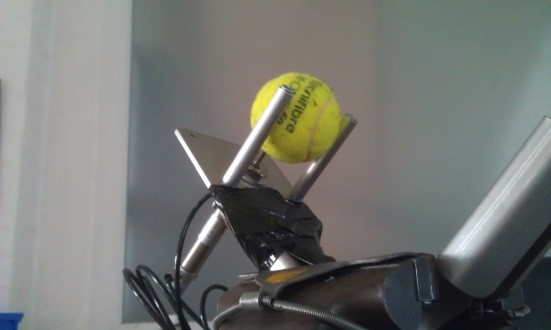
\includegraphics[width=0.8\textwidth]{Funktionstests/Bilder/PneumatikzylinderBild.jpg}
	\centering
	\caption{Funktionsmuster Pneumatikzylinder} 
\label{abb:PneumatikzylinderBild}
\end{figure}